%Start
%
%
%******************************************************************************************************%
%                                 Smith diagramm construction                                          %
%******************************************************************************************************%
% Illustrate the construction of smith's diagramm from                      													 %
%******************************************************************************************************%
% Version 1,                                                                                           %
% 07.07.2023                                                                                           %
% L.Lentz@umwelt-campus.de                                                                             %
%******************************************************************************************************%
%
%
\documentclass[tikz,border=10pt]{standalone}
\usetikzlibrary{calc,intersections}
%
\begin{document}
%
\tikzset{
points/.style = {circle,draw,fill=white,, minimum size=0.6cm,
              inner sep=0pt, outer sep=0pt},
}
%
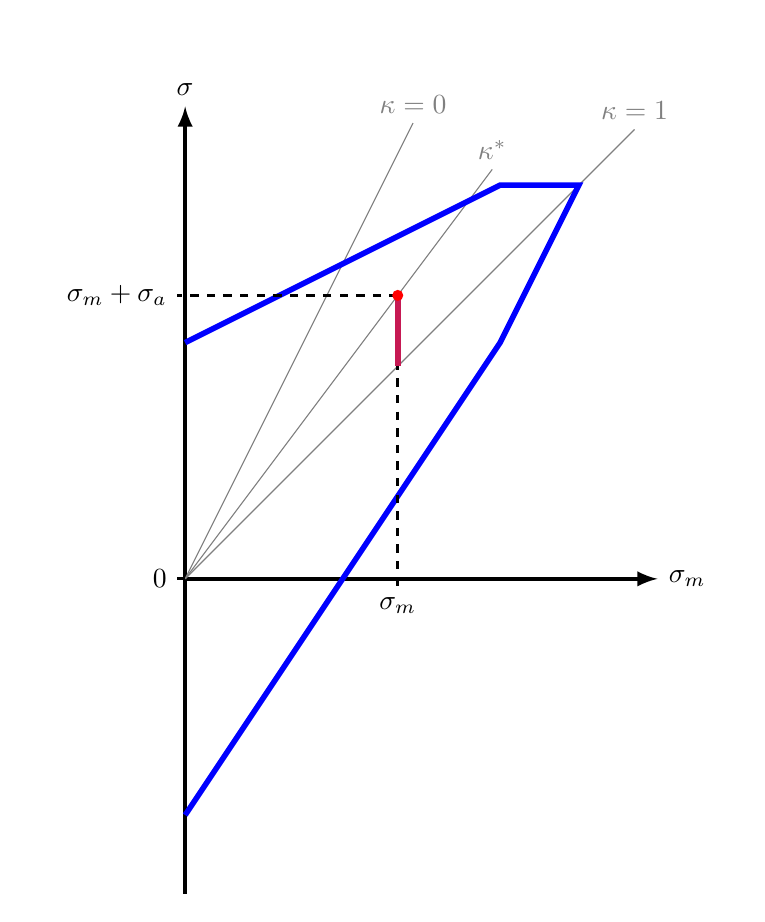
\begin{tikzpicture}
%
\def\delta{1};
\def\os{0.1};
\def\hw{1pt};
\def\lw{1.5pt};
\def\sw{2pt};
%
\def\scal{1/100};
\def\sigw{300*\scal};
\def\sigs{400*\scal};
\def\sigsx{0.5*\sigs};
\def\re{500*\scal};
%
\def\sigm{270*\scal};
\def\siga{90*\scal};
%
\clip[](-2*\delta,-\sigw-\delta) rectangle (\re+2*\delta,\re+2*\delta);
%
\coordinate (O) at (0,0);
\coordinate (Y) at (0,\re+\delta);
\coordinate (X) at (\re+\delta,0);
%
\coordinate (A) at (0,\sigw);
\coordinate (B) at (\sigsx,\sigs);
\coordinate (C) at (\re,\re);
\coordinate (D) at (\sigsx,0);
\coordinate (E) at (0,-\sigw);
\coordinate (S) at (\sigm,\sigm+\siga);
\coordinate (H3) at (\sigm,\sigm);
\coordinate (H4) at (\sigm,\sigm-\siga);
%
\draw[-latex,line width = \lw](O)--(X) node[at end, right]{$\sigma_m$};
\draw[-latex,line width = \lw]($(O)+(0,-\sigw-\delta)$)--(Y) node[at end, above]{$\sigma$};
%
\draw[color=gray,name path=linesm](O)--($(C)!-1.cm!(O)$)node[at end, anchor = south]{$\kappa=1$};
\draw[color=gray](O)--($(B)!-2.cm!(O)$)node[at end, anchor = south]{$\kappa=0$};
\draw[color=gray](O)--($(S)!-2.cm!(O)$)node[at end, anchor = south]{$\kappa^*$};
%
\draw[draw=none,name path=line1]($(C-|O)+(-\os,0)$)--(C);
\draw[line width=\hw](O)--+(-\os,0)node[at end, left]{$0$};
%
\draw[draw=none,name path=line2](A)--($(A)!+50!(B)$);
\path[name intersections={of=line1 and line2,by=H1}];
%
\draw[draw=none,name path=line3](H1)--+(0,-\re);
\draw[draw=none,name path=line4](E)--($(E)!50!(D)$);
\path[name intersections={of=line3 and line4, by=H2}];
%
\draw[color = blue,line width = \sw](A)--(H1)--(C)--(H2)--(E);
%
%\coordinate (H3) at (intersection of $(S|-O)$--S and O--C);
%
\draw[dashed,line width=\hw](S)--($(S-|O)+(-\os,0)$)node[at end,left]{$\sigma_m+\sigma_a$};
\draw[dashed,line width=\hw](S)--($(S|-O)+(0,-\os)$)node[at end,below]{$\sigma_m$};
\draw[color=purple!90,line width=\sw](H3)--(S);
\draw[fill=red,draw=none] (S) circle (2pt);
%
\end{tikzpicture}
%
\end{document}
%
%
%
%End